\section{Einleitung}
In letzter Zeit hat sich das Sortier- und Suchverhalten der Menschheit geändert. Sortierte man früher noch seine Dokumente in Ordner, ist man heute glücklich, wenn man mit leistungsstarken Suchalgorithmen schnell und präzise das gewünschte Dokument findet.\\
Dabei beschränken sich Suchanfragen nicht nur auf lokale Daten, sondern werden sogar großteils ans Web gestellt. Eine häufige Anfrageform an Suchmaschinen sind hierbei die \textit{named entity queries}\cite{paper:Guha}.\\
\begin{figure}[h]
	\centering
	\begin{tabular}{c}
		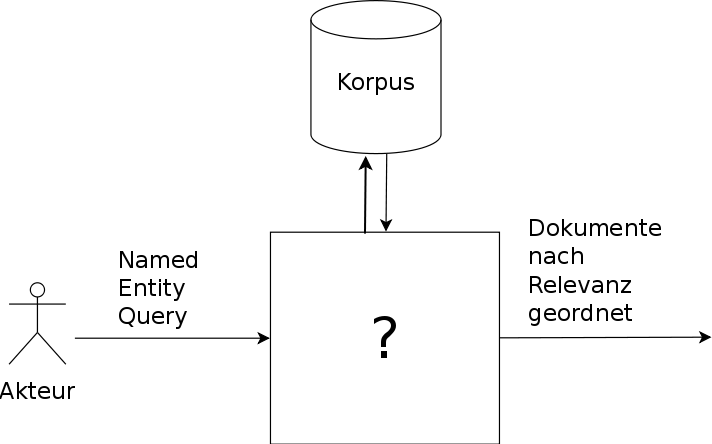
\includegraphics[scale=.2]{pics/overview}
	\end{tabular}
	\caption{Häufige Suchanfrage an Suchmaschinen}
	\label{tab:freq_query}
\end{figure}\\
Ein Problem bei solchen Suchanfragen ist es, die Häufigkeit der \textbf{named entity} in Dokumenten richtig zu erfassen\cite{paper:Na}.
Denn die Referenzierung des Objektes, das sich hinter einem Eigennamen verbirgt, wird sowohl mit dem Eigennamen selbst, als auch mit kompakteren Ausdrücken vorgenommen.\\
So wird beispielsweise in einem Text, der von Peter Chen handelt, die Person \textit{Peter Chen} auch mit \textit{"`er"'} referenziert.\\
\\
\fbox{ 
\begin{minipage}{12cm}
	"`\textbf{Chen} has recieved serveral awards in the fields of Information Technology. \textbf{He} received the Data Resource Management Technology Award [\ldots]"' \cite{wiki:peter_chen}
\end{minipage}
}\\
\\
In der folgenden Hausarbeit wird ein statistisches Verfahren erklärt, welches die Häufigkeit von Eigennamen in Dokumenten schätzen soll. Grundlage für diese Ausarbeitung ist ein Paper der Herren Na und Ng über "`A 2-Poisson Model for Probabilistic Coreference of Named Entities for Improved Text Retrieval"'\cite{paper:Na}.

